% Fig 3.17 Hyperfine structure of an ESR line for J=5/2, I=5/2 (e.g. Mn2+):
% six m_J groups, each split into six hyperfine lines (E = g mu_B B m_J + A m_I m_J);
% 30 slightly tilted double-headed transition arrows between adjacent groups.
\documentclass[tikz,border=5pt]{standalone}
\usetikzlibrary{arrows.meta}
\usepackage{amsmath}
\usepackage{bm}
\usepackage{fontspec}
\setmainfont{Times New Roman}
\begin{document}
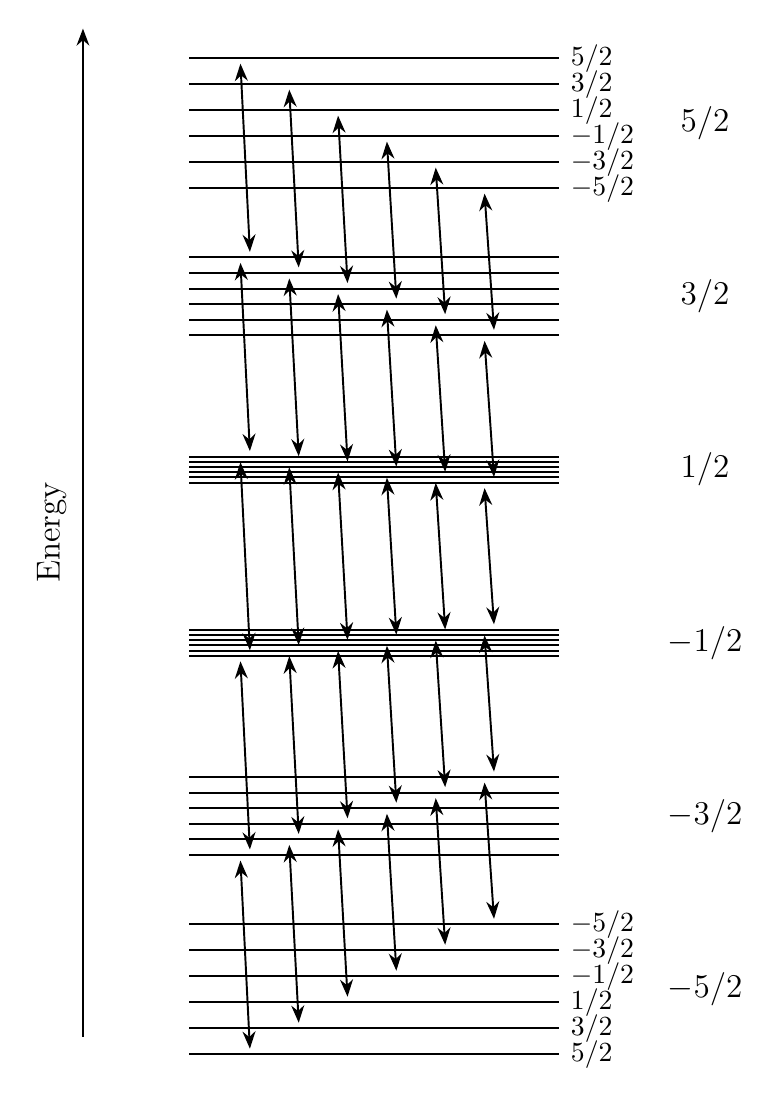
\begin{tikzpicture}[line width=0.7pt,>=Stealth]
\def\A{0.06}      % hyperfine constant in units of the Zeeman group spacing
\def\Xa{1.9}\def\Xb{6.6}
% ---------- level lines: six groups of six ----------
\foreach \mJ in {2.5,1.5,0.5,-0.5,-1.5,-2.5}{
  \foreach \mI in {2.5,1.5,0.5,-0.5,-1.5,-2.5}{
    \pgfmathsetmacro{\y}{(\mJ+\A*\mJ*\mI)*2.2+7.2}
    \draw (\Xa,\y) -- (\Xb,\y);
  }
}
% ---------- small m_I labels on top (m_J=5/2) and bottom (m_J=-5/2) groups ----------
\foreach \mI/\lab in {2.5/{5/2},1.5/{3/2},0.5/{1/2},-0.5/{-1/2},-1.5/{-3/2},-2.5/{-5/2}}{
  \pgfmathsetmacro{\yT}{(2.5+\A*2.5*\mI)*2.2+7.2}
  \node[anchor=west,inner sep=1pt] at (\Xb+0.10,\yT) {$\lab$};
  \pgfmathsetmacro{\yB}{(-2.5-\A*2.5*\mI)*2.2+7.2}
  \node[anchor=west,inner sep=1pt] at (\Xb+0.10,\yB) {$\lab$};
}
% ---------- large m_J labels at right ----------
\foreach \mJ/\lab in {2.5/{5/2},1.5/{3/2},0.5/{1/2},-0.5/{-1/2},-1.5/{-3/2},-2.5/{-5/2}}{
  \pgfmathsetmacro{\y}{\mJ*2.2+7.2}
  \node at (8.45,\y) {\large$\lab$};
}
% ---------- transition arrows (Delta m_J=1, Delta m_I=0), double-headed ----------
\foreach \mJu/\mJl in {2.5/1.5,1.5/0.5,0.5/-0.5,-0.5/-1.5,-1.5/-2.5}{
  \foreach \k/\mI in {0/2.5,1/1.5,2/0.5,3/-0.5,4/-1.5,5/-2.5}{
    \pgfmathsetmacro{\yu}{(\mJu+\A*\mJu*\mI)*2.2+7.2}
    \pgfmathsetmacro{\yl}{(\mJl+\A*\mJl*\mI)*2.2+7.2}
    \pgfmathsetmacro{\xk}{2.55+0.62*\k}
    \draw[{Stealth[length=2.2mm]}-{Stealth[length=2.2mm]}]
      (\xk,\yu-0.07) -- (\xk+0.12,\yl+0.07);
  }
}
% ---------- Energy axis ----------
\draw[->] (0.55,1.1) -- (0.55,13.9);
\node[rotate=90] at (0.15,7.5) {\large Energy};
\end{tikzpicture}
\end{document}
